\section{Sono}

O sono é um processo fisiológico crucial para a consolidação e manutenção das memórias~\cite{blissittSleep2001, walkerSleep2006,
diekelmannMemory2010}. Inicialmente, postulava-se que o sono desempenhava uma função passiva no processo de consolidação da
memória~\cite{jenkinsObliviscence1924}; contudo, com a descoberta das distintas fases do sono, começaram-se a explorar as
contribuições ativas do sono na consolidação mnemônica~\cite{aserinskyRegularly1953}.

O sono possui 5 fases no total, ilustradas na Figura~\ref{fig_fases}, diferenciadas por suas características distintas de
atividade elétrica cerebral, conforme medido por eletroencefalogramas (EEG)\cite{silberVisual2007}: vigília (acordado), N1, N2, N3
e REM (\textit{Rapid Eye Movement}).\@As fases N1 a N3 são conhecidas como sono não-REM (NREM). Ao cair no sono, a fase N1 é a
primeira a ser atingida, seguida por N2, N3, N2 novamente e, por fim, REM;\@esse ciclo se repete ao longo da noite, com cada ciclo
durando aproximadamente de 90 a 110 minutos~\cite{k.patelPhysiology2022}.

\begin{figure}[!ht]
\caption{Fases do sono.}
\centering{
\parbox{12cm}{
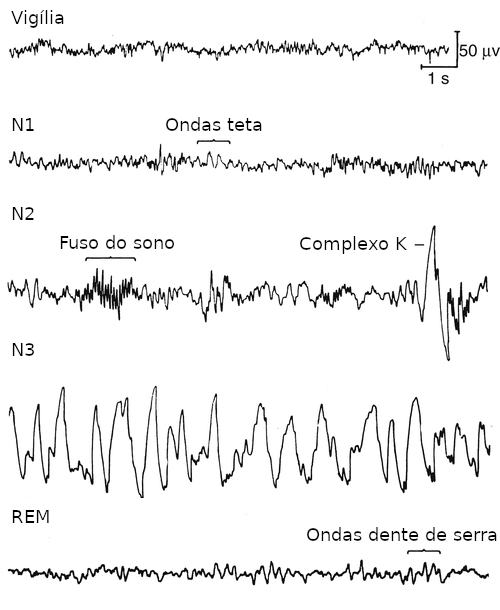
\includegraphics[width=12cm]{figuras/fases_sono.png}\label{fig_fases}
\fonte{\cite{heuerHeuer2021}. Modificada pelo autor.}}}
\end{figure}

Durante o sono NREM, as oscilações lentas geradas no córtex promovem uma comunicação bidirecional entre o córtex e o hipocampo,
facilitando a transferência de memórias do hipocampo, onde são inicialmente codificadas, para locais de armazenamento de longo
prazo no neocórtex~\cite{diekelmannMemory2010}. Esta transferência de memórias é suportada pelos fusos do sono que ocorrem durante
a fase N2, que estão associados à plasticidade sináptica e são cruciais para a estabilização das memórias durante o
sono~\cite{raschReactivation2008, peyracheMechanism2020}.

O estágio REM é quando ocorre a maior parte dos sonhos. O sono REM é caracterizado por atividade elétrica cerebral rápida e de
baixa amplitude, similar àquela observada durante o estado de vigília. A dificuldade em isolar a atividade neural dessa etapa
específica, torna a discussão sobre sua contribuição para a consolidação da memória ainda controversa. Contudo, evidências
recentes sugerem que o sono REM também pode facilitar a consolidação da memória espacial e contextual, bem como a regulação
emocional~\cite{payneSleep2012, boyceREM2017}.

A pesquisa sobre a neurobiologia do sono e da memória ainda está em andamento, e ainda não se sabe porque o sono é tão essencial
para a vida em mamíferos, e novas descobertas continuam a esclarecer a complexidade e a importância do sono para a cognição e a
saúde geral.
